\documentclass[11pt]{report} % Dokumentenklasse

\usepackage[utf8]{inputenc} % Textkodierung: UTF-8
\usepackage[T1]{fontenc} % Zeichensatzkodierung

\usepackage[ngerman]{babel} % Deutsche Lokalisierung
\usepackage{graphicx} % Grafiken
\usepackage[absolute]{textpos} % Positionierung

% Schriftart Helvetica:
\usepackage[scaled]{helvet}
\renewcommand{\familydefault}{\sfdefault}

\usepackage{calc} % Berechnungen
\usepackage{tabto} % Tabulatoren
\usepackage{parskip}
\usepackage{amsfonts}
\usepackage{amsmath}
\usepackage{xcolor}
\usepackage[backend=biber,sorting = none, style=numeric-comp, doi=false, isbn = false, url=false, giveninits=true]{biblatex}
\bibliography{Bibliography.bib}

\usepackage{pgfplots}
\pgfplotsset{compat=1.8,width = 5.5cm}
\usepgfplotslibrary{fillbetween}
\usepgfplotslibrary{groupplots}
\usepackage{pgfplotstable}
\usetikzlibrary{external}
%\tikzexternalize[prefix=./tikz/]


% Debugging:
%\usepackage{layout} % Layout-Informationen
%\usepackage{printlen} % Längenwerte ausgeben




\title{research internship report}
\date{2018-28-01}
\author{Seppich,Nicolas}

%%%%%%%%%%%%%%%%%%%%%%%%%%%%%%%%%%%%%%%%%%%%%%%%%%%%%%%%%%%%%%%%%%%%%%%%%%%%%%%%
% EINSTELLUNGEN
%%%%%%%%%%%%%%%%%%%%%%%%%%%%%%%%%%%%%%%%%%%%%%%%%%%%%%%%%%%%%%%%%%%%%%%%%%%%%%%%

% Seitenränder:
\newcommand{\SeitenrandOben}{43.5mm}
\newcommand{\SeitenrandRechts}{20mm}
\newcommand{\SeitenrandLinks}{20mm}
\newcommand{\SeitenrandUnten}{10mm}

\newcommand{\UniversitaetLogoBreite}{19mm}
\newcommand{\UniversitaetLogoHoehe}{1cm}

\usepackage[a4paper,
    top=\SeitenrandOben,
    bottom=\SeitenrandUnten,
    inner=\SeitenrandLinks,
    outer=\SeitenrandRechts,
    foot=0cm,
    head=0cm
]{geometry}

\textblockorigin{\SeitenrandLinks}{\SeitenrandOben} % Ursprung für Positionierung

\setlength{\parindent}{0pt}
%\setlength{\baselineskip}{32pt}
\setlength{\parskip}{\baselineskip}
\TabPositions{4cm}
\pagestyle{empty}


%%%%%%%%%%%%%%%%%%%%%%%%%%%%%%%%%%%%%%%%%%%%%%%%%%%%%%%%%%%%%%%%%%%%%%%%%%%%%%%%
% DOKUMENT
%%%%%%%%%%%%%%%%%%%%%%%%%%%%%%%%%%%%%%%%%%%%%%%%%%%%%%%%%%%%%%%%%%%%%%%%%%%%%%%%
\newcommand{\Titel}{%
    Titel der Arbeit}
\newcommand{\Untertitel}{%
    Untertitel}
\newcommand{\Grad}{%
    B.Sc./M.Sc. ...}
\newcommand{\Fakultaet}{%
    Fakultät für Muster}
\newcommand{\BetreutVonPerson}{%
    Univ.-Prof. Dr. Dr. h. c. mult. Max Musterprofessor}
\newcommand{\BetreutVonLehrstuhl}{%
    Lehrstuhl für Musterlehre}
\newcommand{\EingereichtVon}{%
    Martin Mustermann\\
    Musterweg 20\\
    80999 München\\
    +49 89 123 456 89}
\newcommand{\EingereichtAmDatum}{%
    Datum}
\newcommand{\ErklaerungUeberschrift}{%
    Anhang I}
\newcommand{\Ort}{%
    Ort}
\newcommand{\Datum}{%
    Datum}

\begin{document}


\begin{textblock*}{\UniversitaetLogoBreite}[1,0](\textwidth-1mm, 2cm-\SeitenrandOben)%
    \raggedleft
\includegraphics{./Deckblatt/Ressourcen/Universitaet_Logo_RGB.pdf}%
\end{textblock*}


\begin{textblock*}{\textwidth}[0,0](0cm, 0cm)%
{\fontsize{24pt}{26pt}\selectfont\textbf{\Titel}}

\vspace*{14pt}
{\fontsize{18pt}{27pt}\selectfont\textbf{\Untertitel}}
\end{textblock*}

\vspace*{92.2mm}
\fontsize{15pt}{17.5pt}\selectfont%
Wissenschaftliche Arbeit zur Erlangung des Grades\\
\Grad\\
an der \Fakultaet{} der Technischen Universität München.

\renewcommand{\baselinestretch}{1.47}
\normalsize\selectfont
\vspace*{17.1mm}
\textbf{Betreut von}\tab
\begin{minipage}[t]{\textwidth-\CurrentLineWidth}
\BetreutVonPerson\\
\BetreutVonLehrstuhl\strut
\end{minipage}

\vspace*{4.3mm}
\textbf{Eingereicht von}\tab
\begin{minipage}[t]{\textwidth-\CurrentLineWidth}
\EingereichtVon
\end{minipage}

\vspace*{-1mm}
\textbf{Eingereicht am}\tab 
\begin{minipage}[t]{\textwidth-\CurrentLineWidth}
München, den \Datum\strut
\end{minipage}

\newpage

\vspace*{-15.8mm}
\fontsize{19pt}{21pt}\selectfont
\ErklaerungUeberschrift

\vspace{25.3mm}
Erklärung

\normalsize\selectfont
\vspace{13.2mm}
Ich versichere hiermit, dass ich die von mir eingereichte Abschlussarbeit selbstständig verfasst und keine anderen als die angegebenen Quellen und Hilfsmittel benutzt habe.

\vspace{18.1mm}
\rule[-3.7mm]{\linewidth}{0.5pt}
\Ort{}, \Datum{}, Unterschrift


{\bf Style guide}
\begin{itemize}
\item Treat equations as sentences, that is end them with point or comma's, so that it integrates with the text.
\item Focus on the content of the report, not the layout. That is for, don't try to force latex to have spacing at each paragraph. It is better to do this at the end, so you can programmatically perform these adjustments.
\item You have to ease the reader into the subject, assume that the person reading the text doesn't know anything about the report. Try to read it using this mindset and reflect if you would be able to follow your report when you had read it for the first time
\item Try to write it, so that you also enjoy it to read. If you don't enjoy it to read, don't expect that anyone else will like it either!
\end{itemize}
{\bf Suggestions for change}
\begin{itemize}
    \item Chapter 1 Preface and acknowledgment: Give here information on what you need the do for your university, why you choose the KTH and your part within the IMAGE project (keep the part about IMAGE short, there will be info later).
    \item Chapter 2 Introduction. Write here the background to the problem that you have looked at and explain the research objective.
        \begin{itemize}
            \item Background: Introduce the concept of acoustic liners, the measurement of their properties, connection with IMAGE and also introduce the prony method in words. Show that it works only for a equispaced grid. 
            \item Problem: Determine uncertainty in results obtained using Prony-like methods
            \item Objective: Introduce the use of non-equispaced grids
        \end{itemize}
    \item Chapter 3 Theory: Introduce here the information needed to understand the problem that you have worked on and focus on the approximation. Try to line up your writing with the code that you have used.
    \item Chapter 4 Results and conclusion
        \begin{itemize}
            \item Numerical experiments: Show here the results that you have obtained using your code and the error analysis that you have done.
            \item Experimental results: Show here the results that you have obtained using the uncertainty analysis.
        \end{itemize}
\end{itemize}


\maketitle
\pagenumbering{gobble}
\newpage
\pagenumbering{arabic}

\setcounter{secnumdepth}{5}
\chapter{Preface}
\section{Motivation}
Studying at university at undergraduate level usually means to a lot of students to study most of the time on a pure theoretical basis.
But since working in academia is supposed to combine both practical experimental and purely theoretical work, my department of the Technical University Munich provides the opportunity to gain insights into research topics during an optional research internship.
As part of my curriculum in engineering science at the Munich School of Engineering, I decided to complete this internship at the Marcus Wallenberg Laboratory for Sound and Vibration of the KTH in Stockholm, Sweden in the field of aero acoustics-
more specifically in the field of passive noise reduction using acoustic liners in aircraft engines. Here, I participated in a research project named the IMAGE project focussing on the optimization of these liners. 
During the 6 weeks of the internship, I could support the researchers and gain a lot of insights in specific tasks, which I am going to present in the following pages. 

\section{My field of activity} 
As the duration of the research internship was limited to period of 6 weeks, I participated in many tasks supporting the researchers instead of completing a single separate task.
These tasks are going to be explained in a detailed way in the following pages, but all in all encompassed the setup of experiments, research in literature, post processing the obtained data numerically with different methods and conducing uncertainty estimates.
I worked both practically in the laboratory and theoretically on fundamental theories of acoustics and maths.
As a member of a team of 3, I could also benefit from the expertise of my colleagues as well as acquiring helpful skills in team working. 

\subsection{Gathering of information concerning acoustics } 
The first days of the internship were used to acquire the demanded knowledge about acoustics, its governing equations and its methodologies.
In order to fulfil this purpose, the main task was to read several books such as 1, 2, 3 and gather serveral articles concering the topic of acoustics, especially in flow acoustics. 
After a short period, I realized, that flow acoustics govers the combination of different subjects, which I already passed at TUM such as continuum mechanics, signal processing, control theory and thermodynamics.
With the acquired knowledge I was able to pass on to the main tasks. 

\subsection{Conduction of measurement series}
As I also participated in measurement series, several tasks needed to be fulfilled.
This included the preparation of the test setup, preparation of the acoustical liners, callibration of the microphones and the conduction of test with or without flow.
Conducting these different steps in a specific order helped me to get a better understanding in how scientific tests are organized and which details need to be considered in order to get precise results. 

\subsection{Development of the equispacing algorithm}
Basically my main task to be completed during the internship, was the development of an algorithmn to postprocess the data obtained by the measurement in a special way. 
The purpose of the implemented algorithm is to approximate a function at equispaced positions to meet the basic requirements for further postprocessing steps as determining the impedance numerically or using uncertainty estimate techniques to obtain reliable results.  
In order to fulfill this specific purpose, I conducted quite a lot of literature research to understand the governing background theory in the field of nonlinear approximation.
Several papers served as reference for the implementation of the algorithm. 
Due to the complexity this specific task consumed most of time during the internship.
In chapters 3 and 4 I will outline the algorithm and the obtained results in a more detailled way.
 
\chapter{Introduction} 
As acoustics is field of studies that bother our everyday lives, it is important to distinguish between wanted and unwanted acoustics.
While on one side acoustics are highly appreciated and essential in the field of communication, noise on the other side, is an unwanted side effect of many technical applications and can even lead to severe consequences for people.
Therefore, it is essential to develop efficient ways to reduce noise.

\section{Acoustic liners for passive sound reduction}
The research project, where I had the chance to get insights in during my internship, covered the topic of passive noise reduction methodologies with acoustic liners in aircraft engines.
In general, acoustic liners are components to damp imcoming sound waves using the principle of Hemholz resonance to dissipate energy.
In aircraft engines the aeroacustic liners are placed within the two critcal areas of the engine - in the inlet and in the outlet, where most of the noise is generated. 	 
The principle set up of a liner consists of a porous or perforated top layer, a honeycomb structure and an impervious layer. 
Since the fundamental principle of passive noise reduction with sound absorbing materials in liners has been used for a long time, the focus is set on the optimization of several set ups and liner designs.


\section{The IMAGE project} 
In aero- engines, single-layer and double-layer liners with perforate and mesh facing sheets are standard elemtents to reduce noise, but for the optimization of novel liner designs and novel materials more research is required to understand their acoustic impedance characteristics.
This is where the project IMAGE comes into play.
The term IMAGE stands for Innovative Methodologies and technologies for reducing Aircraft noise Generation and Emission.
In detail, the project aims to investigate noise reduction technologies in aircrafts both in a numerical and experimental way in order to develop robust methodologies in this particular field of study.  
Whereas the main goal of the study conducted at the KTH at the Marcus Wallenberg Laboratory covers the characterization of the acoustical behaviour of porous materials in the reduction of fan noise in duct flow. 
The obtained results provide the  basis references for further optimization steps of liners or for the further validation of numerical methods. 

\section{Characterisation of the impedance of liners in duct flows}
The experiments conducted at the MWL aim to determine the impedance spectra and consequently the acoustical behaviour of acoustic liners embedded in the walls of aero- engines.
Therefore, a model that simulates the sound spectrum of a fan in a duct flow is set up. 
The measured pressure provides the basis for post processing steps like the prony method to examine parameters to deduce the impedance.
In order to understand further relations, the experimental setup and fundamental theories are shortly introduced in this section. 


\subsection{Experimental setup and measurements}
In our case, the experimental setup consists mainly of a rectangular duct with the liners embedded into the wall.
With the help of 16 microphones and two loud speakers, that generates the sound field of specific frequencies, the impedance of the liners can be deduced using an inverse analytical method.
In this context, inverse analytical method means to deduce the acoustical impedance by measuring the sound field in a mean flow, in front of and after the lined section.
Therefore, 3 microphones and one speaker are placed respectively in front of and after the lined section, whereas the remaining 10 microphones face the the liner.
The method is a non destructive method ensuring the liners further usage.
The governing relation between the measured pressures and how to determine the impedance is going to be presented more detailled later on. 

Graph Experimental setup
	

\subsection{The wave equation and its solutions}
Acoustic phenomena are based on wave propagation. As a consequence the coverning equation is called the wave equation and is of the form: 

\begin{equation}
\nabla^2p-\frac{1}{c^2}\frac{\partial^2p}{\partial^2t}
\end{equation}. 

There are several ways to derive this partial differential equation including conservations laws like mass and momentum conservation, which are the fundamental equations in thermodynamics and mechanics. 
Using complex notation the equation becomes: 

\begin{equation}
\nabla^2 \hat{p}-k^2 \frac{\partial^2\hat{p}}{\partial^2t}
\end{equation},  

which is called the Helmholz equation, where $k=\frac{w}{c}$ denotes the wavenumber. 
The Helmholz equation has the general solution:
\begin{equation}
p(x)=p^{-}e^{i(wt-k\textbf{x})}+p^{+}e^{i(wt-k\textbf{x})}
\end{equation}
with x the propagation vector. 

\subsection{Case of a rectangular duct}
In our case of a rectangular duct, the Helmholz equation takes the form: 
\begin{equation}
\frac{\partial^2\hat{p}}{\partial x^2}+\frac{\partial^2\hat{p}}{\partial y^2}+\frac{\partial^2\hat{p}}{\partial xz^2}+k^2\hat{p}
\end{equation}
where we used the rectangular coordinate system. 
graph of a duct with coordinate system.
Using the boundary conditions 
\begin{equation}
\left.\frac{\partial\hat{p}}{\partial x}\right\rvert_{x=0,x=a}=0
\end{equation}

\begin{equation}
\left.\frac{\partial\hat{p}}{\partial y}\right\rvert_{y=0,x=b}=0
\end{equation}
leads to following restrictions on the wave numbers 

\begin{equation}
k_{x,m}=\frac{m\pi}{a}
\end{equation}
\begin{equation}
k_{y,n}=\frac{n\pi}{b}
\end{equation}
where n and m denote the different modes of the solution to to wave equation. 
Using this information and the assumption that the solution is of the form: 
\begin{equation}
\hat{p}(x,y,z,t)=p_{x}(x)p_{y}(y)p_{z}(z)e^{iwt}
\end{equation}
leads to the fundamental solution in rectangular ducts: 

\begin{equation} \label{eqn:ductmodes}
\hat{p}(x)=\sum\limits_{m=1}^\infty\sum\limits_{n=1}^\infty \epsilon_{n}\epsilon_{m}\cos(\frac{m\pi x}{a})\cos(\frac{n\pi y}{b})\left( p_{mn}^{+} e^{i(wt-k_{z,mn})}+p_{mn}^{-}e^{i(wt+k_{z,mn})} \right)
\end{equation}

where $\epsilon_{n}$ $\epsilon_{m}$ are the normalisation constants. 
Consequently, the the equation can be separated into two parts. 
The first part describes the shape of the oscillation in the ducts crosssection, whereas the second part describes the propagation term. 
When m=n=0 the equation reduces to the form:
\begin{equation}
p(x)=p^{-}e^{i(wt-kz)}+p^{+}e^{i(wt-kz)} 
\end{equation}, which corresponds to the one dimensional Helmholz equation. 
  

\subsection{Relation between wavenumber and impedance}
If the wavenumber $k_z$ is known,then the impedance $z_{ac}$ can be calculated with following relations:  
\begin{equation}\label{eqn: Impdet1}
    k_y \tan 2k_y H = \frac{i \rho_0 c_0^2}{\omega z_{ac}} \left[k-M_zk_z\right]^2
\end{equation}
and
\begin{equation}\label{eqn: Impdet2}
    k_z = \frac{k}{1-M^2} \left( -M \pm \sqrt{1+(1-M^2)(k_x^2/k^2 + k_y^2/k^2)}\right)    
\end{equation}
$k_z$ is measured, then from the first relation $k_y$ can be obtained under the consideration that the frequency is low enough that there are no modes in the $x$ direction $k_x = 0$, then with the first equation the acoustic impedance $z_ac$ can be obtained.
These solutions are obtained using the considerations of a mean flow M whithin a rectangular duct an d that for the case, that there are no reflections. So the acoustical field consists only of one mode. 


\section{Introduction to the Prony method}
In this section, the already mentioned Prony method is shortly introduced, which aims to recover the signal parameters from noisy sampled data to determine the experimental impedance of the liners.
As shown before in equation (\eqref{eqn:ductmodes}) the acoustic field within the duct consists of acoustic modes. 
Therefore, the Prony method takes a similar model into account, which is of the form: 
\begin{equation}\label{eqn: expsum}
 p(x)=\sum\limits_{j=1}^M c_{j}e^{ik_{j}z} 
\end{equation}
where M denotes the number of acoustical modes. 
So, the problem that the prony method faces  can be considered as a nonlinear approximation problem, where of the  pairwise different wavenumbers $k_{j}$ and complex coefficients $c_{j}$ are recovered.
When the factors $c_j$ and $k_j$ are known, they can be related to the acoustic impedance with the previous equations (\ref{eqn: Impdet1})(\ref{eqn: Impdet2})
For the purpose to solve this problem, there is an algebraic solution, twhich is known as the prony methdod. But there are also various other prony like the Esprit method( Estimation of Signal Prarameters cia rotational Invariance Techniques) or the matrix pencil method described by \cite{Potts}.
In order to calculate the algebraic solution, it is necessary, that the data is sampled at M*2 points, fulfills the Shannon-Nyquist theorem and that the data points are equispaced. 

\section{Problem: Facing uncertainties}
As measured data is always accompanied by uncertainties, it is also of high importance to fit the uncertainty analysis into the basic modelling process.
Normally, this is a problem of non-trivial kind based on the right assumptions.
With the initial situation of only a few measurement points with quasi equispaced distances it is not possible to calculate uncertainties, where derivatives in the following form are demanded:
\begin{equation}
u_{i}(q)= \left\vert \frac{\partial q}{\partial x_{i}} \right\vert u( x_{i})
\end{equation}
where $u_{i}(q)$ denotes the uncertainty in the desired quantity $q$ due to the uncertainty in $x_{i}$.
Using the fact, that the microphone postitions are not perfectly equispaced, allows us to approximate the wanted function at equipaced steps.
Thus, new data points are generated, which are not only necessary to calculate derivatives, but also to use the Prony method, where an equispaced grid is a basic requirement.
For these reasons an algorithm to approximate the function of complex pressure at an equispaced grid needed to be implemented. 
  
\chapter{Theory on the equispacing algorithm} 
As already seen, the approximation of the complex pressure function at an equispaced grid poses a basic requirement for the prony method as well as for using uncertainty estimates on the experimental data.
This is why, this chapter in particular focuses on the implementation and theories behind the equispacing algorithm, beginning with the basic ideas first followed by a detailed review. 

\section{Basic ideas}
The algorithm is based on the theory of \textit{non linear approximation by sums of exponentials and translates}, by \cite{Peter2011}.\\
So basically the idea of the algorithm includes as before in equation \eqref{eqn: expsum} to first approximate the function of obtained complex pressures with a linear combination of complex exponentials.
This makes the approximation to be of the same form as the fundamental solution of the wave equation in a rectangular duct.
Then, assumptions about coefficients help to transform the problem into a linear system of equations. Solving this system in combination with using an equispaced grid lead to the approximation of the complex pressure. 
In the following section the detailed ex

\subsection{Generalization of the approximation}
In this case, we generalize the equation \eqref{eqn: expsum} to a nonequispaced grid, i.e. on the known nodes $x_{k}\in (-\frac{1}{2},..,\frac{1}{2})$ for k $\in{1,..., K}$ with the measured data  $p(x_{k}) $

\begin{equation}
 p(x_{k})=\sum\limits_{j=1}^M c_{j}e^{2\pi ix_{k}Ns_{j}}
\end{equation}
with complex coefficients $c_{j} \neq 0$
\\
Note that $2 \pi Ns_j \in{-\pi N,\pi N}$ are the frequencies of $p(x)$

\subsection{Approximation of the coefficients $c_j$ and determination of the coefficients $p_l$}
In a second step, the complex coefficients $c_j$ are approximated by the fourier transform of a window function, which will be explained later on in deail. 
This transforms the equation to: 

\begin{equation}
\sum\limits_{j=1}^L p_{l}\psi(x_{k}-\frac{l}{L})=p(x_{k})\label{eqn: linear system}
\end{equation}


In a third step, the parameters $p_l$ are going to be recovered solving the linear equation for all nodes.

\subsection{Approximation at the non equispaced grid}
With the obtained coefficients, the approximation will be completed adapting equispaced parameters into the equation (\eqref{eqn: linear system}): 

\begin{equation}
 \sum\limits_{j=1}^L h_{l}\varphi(x'_{k}-\frac{l}{L})=p(x'_{k})\notag
\end{equation}


 



To enhance the understanding of the sequential formulas, the main parameters of the algorithmn are going to be presented in the following:

 K: K is the number of nodes and therefore the number of rows in the following linear equation\\
 N: N is the nonharmonic Bandwidth\\
 L: L is the number of exponentials to approximate the function


But in order to recover the parameters of the sum,the signal must be brought into the form first:  
\begin{equation}\label{eqn:truncatedw}
 p(x)=\sum\limits_{j=1}^M h_{l}\psi(x-\frac{l}{L})
\end{equation}

Where $\psi$ denotes the so called truncated window function with many helpful properties such as to be localised well in space and time, which will be discussed later more detailed. \\

\paragraph{Window functions	} $ $\\[1ex]
In general, a function is called a window function, which is zero valued outside a specific chosen interval.
So as one can assume, there are quite a lot of possibilities to set up these window functions.
For our case the 1- periodization of a gaussian bell, as proclaimed in the paper of Steidl seemed to provide good results to work on with.
It is of the form: 

For a fixed $b>0$ and L let:
\begin{equation}
\varphi(x)= \frac{1}{\sqrt{\pi b}} \sum\nolimits_{r \in \mathbb{N}}  e^{(L(x+r))^2/b}
\end{equation}
The truncated version of the gaussian bell takes the form: 
\begin{equation}
\psi(x)= \frac{1}{\sqrt{\pi b}} \sum\nolimits_{r \in \mathbb{N}}  e^{(L(x+r))^2/b}\chi_{(-m,m)}(L(x+r))
\end{equation}
with $1<m < \frac{L}{2}$ and
\begin{equation}
    \chi_{(-m,m)}(x)=
    \begin{cases}
      0, & \text{if}\ x\in (-m,m) \\
      1, & \text{otherwise}
    \end{cases}\notag
\end{equation} 
The question arose, why do we need to truncat the Gaussian bell? In the end, this is a mathematical trick to be well localized in space and time, which allows further mathematical proofs, that are not examined in this report further on.

So, after setting up the truncated window function we are able to solve the linear systems of equations of this form:
\begin{equation}
\sum\limits_{j=1}^L h_{l}\psi(x_{k}-\frac{l}{L})=p(x_{k})
\end{equation}
This can be written in a linear system of equations, which can be solved easily. {\color{red} You could write the matrix equation, just to make it easier to follow}
Here, we aim to examine the coefficients $h_{l}$, which will be used in the second step to approximate the function on the equispaced grid at the specific positions.
The grid can be equalized, using a simple algorithm, which examines the average step size and generates a new grid with this information.
With all coefficients $h_{l}$ and equipspaced positions $x'_{l}$ it is now possible to examine to approxiamte the complex pressure at the equispaced grid. 
\begin{equation}
 \sum\limits_{j=1}^M h_{l}\psi(x'_{k}-\frac{l}{L})=p(x'_{k})\notag
\end{equation}

\paragraph{Results using the truncated window function} $ $ \\[1ex]
In the following, the results of this specific method are going to be discussed.
The parameters where chosen by formulas presented by Peter: \\
	(formulas for parameters) \\
	(graphs)
As the results show, the approximation of the function worked well within the domain, but diverged on the boundaries.
So, using the truncated window function in this specific case was not the optimal solution. \\[1ex]

\paragraph{Approximation with a single Gaussian Bell}  $ $ \\[1ex]
The major goal of the algorithm is to approximate the function of complex pressures as good as possible.
Due to the fact, that every function can be approximated by almost any function, we slightly changed our startin function \eqref{eqn:truncatedw} {\color{red} Why? Explain!} and simply used this form of the original gaussian window function: 
\begin{equation}
 p(x)=\sum\limits_{j=1}^L h_{l}\varphi(x-\frac{l}{L})
\end{equation}
with $\varphi$ is the orignal gaussian bell function: 
\begin{equation}
\varphi(x)= \frac{1}{\sqrt{\pi b}}  e^{x^2/b}
\end{equation}
where l denotes the shift parameter.

In essence, the rest of the main algorithm remained basically the same.
It is still the goal to deduce the coefficients $h_{l}$ by solving the linear system of equations: 
\begin{equation}
\sum\limits_{j=1}^L h_{l}\varphi(x_{k}-\frac{l}{L})=p(x_{k})
\end{equation}
and then approximate the function with remained coefficients at the equispaced grid: 
\begin{equation}
 \sum\limits_{j=1}^L h_{l}\varphi(x'_{k}-\frac{l}{L})=p(x'_{k})\notag
\end{equation}
Again, the algorithm needed to be verified under realistic values and under a nonequispaced grid. A testclass with possible numbers of scenerios. 
During the test cases with using error estimation techniques, it could be examined that the algorithm fulfilled the proclaimed purpose as long as the nonequispacing was not set to random {\color{red} If you have information on the limitations of the mind, include it! This will strengthen your belief that it works for the cases for which we are using the algorithm for}
\cite{Peter2011}
\cite{Mungur1969}
\printbibliography

\chapter{results and conclusion}

\begin{figure}[b]% Reflection coefficient   
    \centering
    \begin{tikzpicture}[scale = 1]
        \begin{axis}[
                xlabel={Frequency [kHz]},
                ylabel={$|\hat{\mathcal{R}}|$ [-]},
                axis on top,
                xmin = 0, xmax = 4,
                ymin = 0.96, ymax = 1,
                minor tick num = 5,
                grid
            ]
            \addplot[
                    color =  red,
                    line width = 0.5,
                ] 
                table[x expr= \thisrow{f}/1000, y={mag} ] {./Data/UncertaintyAnalysis.txt};
            \addplot[line width = 1] table[x expr= \thisrow{f}/1000, y={create col/linear regression={y=mag}}] {./Data/UncertaintyAnalysis.txt};
        \end{axis}
    \end{tikzpicture}
    \begin{tikzpicture}[scale = 1]
        \begin{axis}[
                xlabel={Frequency [kHz]},
                ylabel={$\angle \hat{\mathcal{R}}$ [deg]},
                axis on top,
                xmin = 0, xmax = 4,
                ymin = -5, ymax = 5,
                minor tick num = 5,
                grid
            ]
            \addplot[
                    color =  black!90,
                    line width = 0.5,
                ] 
                table[x expr= \thisrow{f}/1000, y={phase} ] {./Data/UncertaintyAnalysis.txt};
        \end{axis}
    \end{tikzpicture}
    \caption{Measured reflection coefficient of the rigid plate. In blue the measured value and red gives the 95\% confidence intervals}
    \label{fig:ReflCoeff}
\end{figure} 

\begin{figure}
\centering
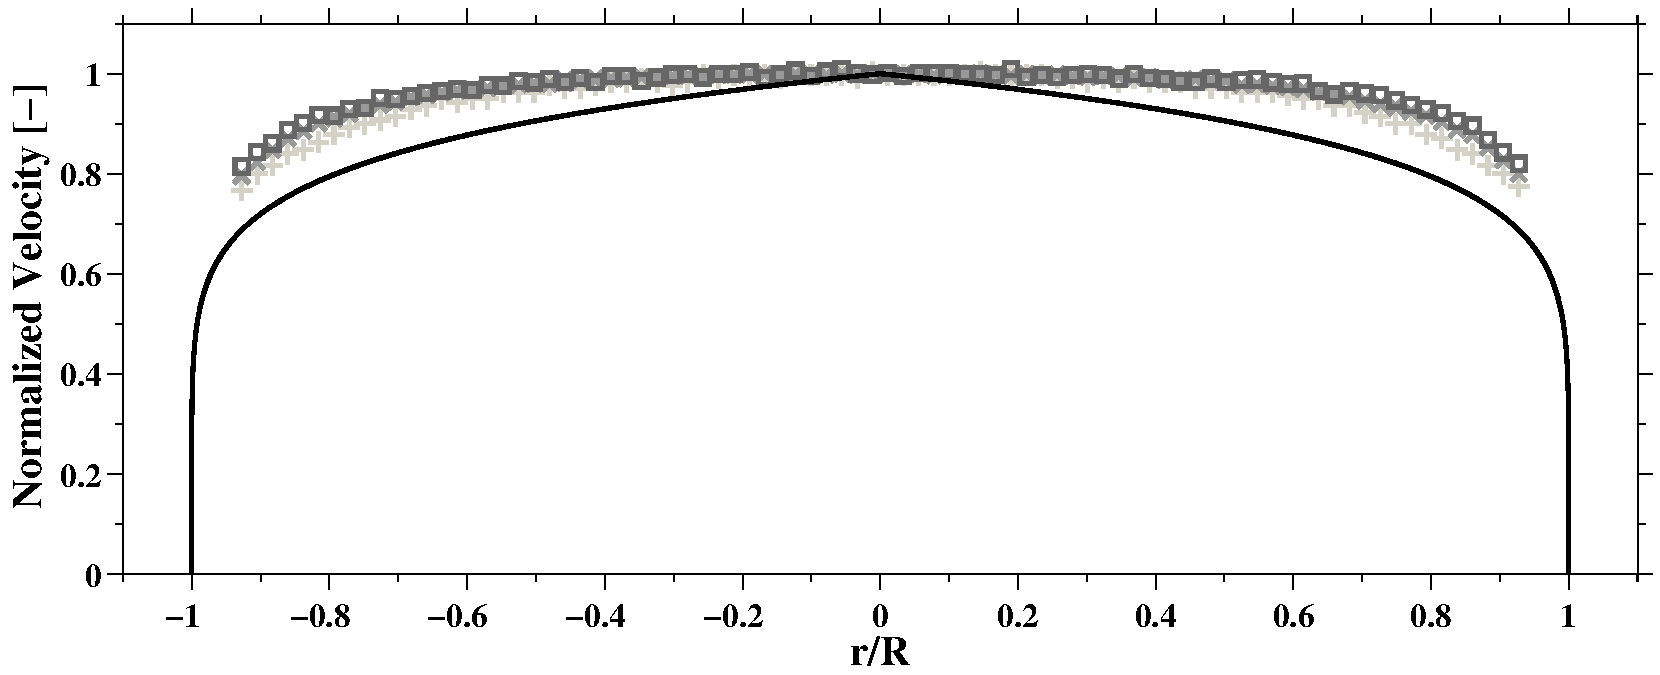
\includegraphics[width = 0.8\textwidth]{./Figures/FlowProfile_Large}
\caption{Test 123}
\end{figure}


\end{document}


